\documentclass[journal]{IEEEtran}

\usepackage{graphicx}
\usepackage{amsmath,amssymb,amsfonts} 
\usepackage{booktabs}                 
\usepackage{cite}                 
\usepackage{url}
\usepackage{bbm}
\usepackage{algorithm}
\usepackage{algorithmic}
\usepackage{float}
\usepackage{placeins}
\usepackage{subcaption}

\graphicspath{{assets/figures/}}

\ifCLASSINFOpdf
\else
\fi

\title{Camera-Observable Multi-Agent Reinforcement Learning for Traffic Signal Control in Mixed Motorcycle-Dominant Traffic}

\author{
    Le~Trong~Nghia,
    and~Nguyen~Thien~Bao,~\IEEEmembership{Member,~IEEE}%
\thanks{
    Le Trong Nghia is an undergraduate student in Robotics and Artificial Intelligence Engineering,
    Institute of Intelligent and Interactive Technologies,
    University of Economics Ho Chi Minh City (UEH),
    Ho Chi Minh City 700000, Vietnam
    (e-mail: nghiale.31241024698@st.ueh.edu.vn).
}%
\thanks{
    Nguyen Thien Bao is with the Institute of Intelligent and Interactive Technologies,
    University of Economics Ho Chi Minh City (UEH),
    Ho Chi Minh City 700000, Vietnam
    (e-mail: baont@ueh.edu.vn).
}%
\thanks{
    Corresponding author: Nguyen Thien Bao (e-mail: baont@ueh.edu.vn).
}%
}

\markboth{Submitted to IEEE Transactions on Intelligent Transportation Systems, June~2026}%
{Nghia and Bao: Camera-Observable MARL for Traffic Signal Control}

\begin{document}
\maketitle

\begin{abstract}
Reinforcement learning (RL) for traffic signal control (TSC) typically relies on simulator-privileged states—such as exact queue lengths, per-vehicle waiting times, and precise network arrivals—that no standard roadside camera can provide, thereby creating a critical deployment gap. To bridge this gap, we constrain both the state representation and the reward function strictly to quantities estimable by a commodity traffic camera utilizing standard bounding-box detection and tracking: a 26-dimensional per-agent observation featuring per-approach aggregation and a signed group-mean phase-imbalance feature, alongside a queue-centric vision-proxy reward that combines a mean-of-squares anti-starvation queue penalty with a signed phase-imbalance pressure term and a local region-of-interest (ROI) exit throughput regularizer. The proposed framework is optimized via parameter-shared Multi-Agent Proximal Policy Optimization (MAPPO) with a centralized per-agent-value-head critic and generalized advantage estimation, explicitly trained within a sublane microsimulation environment under a highly heterogeneous, motorcycle-dominant vehicle mix. Evaluated on a 5-junction corridor and a 16-junction grid under time-varying peak demand, the camera-constrained policy reduces mean travel time by [X]\% compared to fixed-time baselines and [Y]\% versus max-pressure actuation, successfully retaining [Z]\% of the performance achieved by a fully privileged-state policy. Furthermore, under a realistic sensing-noise model with error magnitudes empirically measured from the vision detector stack, the control performance degrades gracefully up to twice the calibrated noise envelope, yielding a rigorously measured information-restriction cost of [W]\% relative to the ideal privileged baseline. Ultimately, quantifying the precise cost of restricting multi-agent control to purely camera-computable signals demonstrates that such deployment is practically viable without simulator-privileged sensing; closed-loop field validation is reported in a companion study.
\end{abstract}

\begin{IEEEkeywords}
traffic signal control, multi-agent reinforcement learning, deployability, mixed traffic, sublane model, SUMO.
\end{IEEEkeywords}

\IEEEpeerreviewmaketitle


\section{Introduction}

\IEEEPARstart{U}{rban} traffic congestion imposes severe and compounding economic, environmental, and public-health costs on rapidly growing metropolises. Adaptive traffic signal control (TSC) seeks to relieve this burden by allocating right-of-way in response to real-time demand rather than to a fixed schedule. Over the past decade, deep reinforcement learning (RL) has become the dominant paradigm for adaptive TSC, advancing from single-intersection Deep Q-Networks~\cite{wei2018_intellilight,genders2016_drl}
to pressure-based and cooperative multi-agent formulations~\cite{wei2019_presslight,wei2019_colight,chen2020_mplight}, and most recently to centralized-training, decentralized-execution (CTDE) multi-agent actor--critic methods that coordinate large urban
networks~\cite{yu2022_mappo,mao2023_masac,zhou2024_micdrl,gu2024_partition}. Across this lineage, learned controllers consistently outperform classical fixed-time and actuated heuristics \emph{in simulation}~\cite{wei2019_survey,rltsc_review2025,rltsc_survey2026}. Yet a critical deployment bottleneck persists: almost none of these controllers can be operated on the commodity roadside sensing infrastructure that actually exists at signalized intersections.

\subsection{The Observation Gap, Not the Dynamics Gap}
The principal barrier to deployment is what we term the \emph{observation gap}.
Prevailing RL-TSC frameworks consume simulator-privileged state---exact halting vehicle counts, per-vehicle accumulated waiting times, and network-wide arrival profiles---quantities that a microscopic simulator exposes for free but that no roadside camera can recover at inference time. We deliberately distinguish this
\emph{observation gap} from the \emph{dynamics gap} (discrepancies in the underlying physics or transition delays) that dominates sim-to-real transfer in robotics~\cite{peng2018_dynrand,zhao2020_sim2real_survey} and that recent TSC transfer studies also target~\cite{da2024_promptgat}: the two are orthogonal, and closing one does not close the other. Legacy inductive-loop detectors offer only a partial remedy, since point sensing captures presence but not spatial composition, vehicle class, or continuous speed profiles~\cite{zhang2021_partialdetection}. Camera-based RL-TSC has begun to narrow the state side of the gap by extracting occupancy or queue features from
video~\cite{dai2022_worldmodels,azfar2025_cosim,su2025_visionllm}; however, these works constrain only the \emph{observation} space while still training and evaluating against a \emph{privileged reward} (e.g., simulator delay or network throughput) that is unavailable at the edge. The paired restriction of
\emph{both} state and reward to camera-computable signals therefore remains substantially under-addressed. This paper closes the observation gap by construction and quantifies its restriction cost in simulation; closed-loop physical field operation is reported in a companion study and is explicitly outside the present scope.

\subsection{Challenges}
Engineering an RL-TSC controller that factors entirely through commodity sensing raises three coupled technical challenges.
\emph{(i) Spatial granularity.} A camera region of interest (ROI) measures traffic as an approach-level aggregate and cannot supply the per-lane occupancy indices that classical state formulations presuppose, particularly where lane discipline is weak.
\emph{(ii) Reward unmeasurability.} The most effective RL reward signals---system-wide delay and exact per-vehicle waiting time---are not computable at the edge, so a reward optimized in simulation generally cannot be reproduced at deployment without a privileged read.
\emph{(iii) Heterogeneous traffic dynamics.} In developing metropolises, traffic is heavily motorcycle-dominant and non-lane-based: motorcycles filter and swarm between lanes~\cite{ngoc2021_fivecities,vn_roundabout}, a behavior that 
breaks car-centric, lane-indexed state and reward designs and that demands continuous-space (sublane) microsimulation rather than discrete lane queues.

\subsection{Contributions}
We propose a deployability-constrained multi-agent proximal policy optimization (MAPPO) framework that addresses these challenges through four verifiable contributions.
\begin{itemize}
  \item \textbf{C1 (Camera-computable state proxy).} We design a
  $26$-dimensional per-agent observation built on per-\emph{approach}
  aggregation rather than per-lane indexing. Each approach contributes bounded features (effective queue, occupancy, average speed, motorcycle share, heavy-vehicle share) and the controller state is completed by a phase one-hot vector, a normalized green timer, and a \emph{signed group-mean} pressure scalar. Every feature admits a documented camera estimator from a YOLOv11~\cite{khanam2024_yolov11}
  plus ByteTrack~\cite{zhang2022_bytetrack} pipeline, specified in
  Section~\ref{sec:obs_space} (Table~\ref{tab:obs_space}); its residual recovery error is
  bounded by the sensing-noise model of Section~\ref{sec:noise_model}, with full per-feature
  calibration against labeled ground truth deferred to the companion field study.
  \item \textbf{C2 (Proxy-computable reward).} We formulate a
  \emph{queue-centric} vision-proxy reward
  in which \emph{every} term factors through the same camera projection as the state---no term reads a privileged simulator quantity, the accumulated-delay penalty included. Its congestion core pairs the $L_2$ norm of the per-approach halted-queue signal (a mean-of-squares penalty that discourages starvation via Jensen's inequality) with the $L_1$ norm of the \emph{same} signal (a linearly-averaged delay proxy); this core is regularized by a signed \emph{phase-imbalance} pressure term---an intra-junction demand gradient, distinct from network max-pressure---that supplies a reward gradient even when allocation is correct, and by a local ROI-exit throughput term whose simulator computation is semantically identical to ByteTrack track terminations at an ROI boundary.
  \item \textbf{C3 (Information-restriction cost).} We isolate and quantify the \emph{information-restriction cost} by comparing the proxy-constrained policy against an otherwise-identical privileged-state policy evaluated on pristine features, and we characterize graceful degradation under a sensing-noise model whose magnitudes are set on a documented basis from the detection-and-tracking literature---with the class-confusion rate measured from the detector's own confusion matrix---rather than being arbitrarily assumed (Section~\ref{sec:noise_model}).
  \item \textbf{C4 (Mixed-traffic, multi-junction evaluation).} We report multi-seed evaluations on a $5$-junction corridor and a $16$-junction grid under SUMO's sublane model~\cite{lopez2018_sumo} with a motorcycle-dominant
  ($\approx 73\%$) fleet calibrated to Hanoi field data~\cite{ngoc2021_fivecities,cao_sano_hanoi} and time-varying demand. On the $16$-junction grid the policy improves on every camera-deployable baseline---Webster~\cite{webster1958}, max-pressure control~\cite{varaiya2013_maxpressure}, SOTL~\cite{cools2013_sotl}, and independent PPO~\cite{dewitt2020_ippo}---while remaining statistically indistinguishable from a loop-instrumented gap-actuated controller that exploits per-second in-road sensing unavailable to a camera-only deployment; on the $5$-junction corridor, classical progression control remains superior, and we analyze this reversal as a topology-dependence result that delineates where learned camera-only control pays (Section~\ref{sec:topology}). A sublane-versus-lane cross-evaluation furthermore shows that ignoring mixed-traffic dynamics materially alters policy outcomes.
\end{itemize}
We emphasize that the MAPPO algorithm itself is standard and is not claimed as a methodological contribution; it is the vehicle for evaluating the proposed camera-constrained state and reward formulation.

\subsection{Paper Organization}
The remainder of this paper is organized as follows. Section~II reviews related work and positions our contribution. Section~III formalizes the Dec-POMDP, the camera-computable observation projection, and the feature-estimator validation. Section~IV details the queue-centric vision-proxy reward, the MAPPO architecture, and the sensing-noise model. Section~V describes the experimental setup, networks, demand, baselines, and statistical protocol. Section~VI presents the main comparison, the information-restriction cost, robustness under sensing noise, generalization, and ablations. Section~VII discusses limitations, and Section~VIII concludes.
\section{Related Work}

\subsection{Reinforcement Learning for Traffic Signal Control}
RL-based signal control has progressed from single-intersection deep
Q-networks~\cite{genders2016_drl,wei2018_intellilight} through pressure-based and
cooperative multi-agent designs---PressLight~\cite{wei2019_presslight},
MPLight~\cite{chen2020_mplight}, CoLight~\cite{wei2019_colight}, and earlier
coordinated learners~\cite{vanderpol2016_coordinated}, building on the
max-pressure principle~\cite{varaiya2013_maxpressure}---to centralized-training,
decentralized-execution (CTDE) actor--critic methods such as
MAPPO~\cite{yu2022_mappo} and IPPO~\cite{dewitt2020_ippo}, with recent
IEEE~T-ITS work adding attention-based soft actor--critic
control~\cite{mao2023_masac}, incentive-driven
communication~\cite{zhou2024_micdrl}, constrained
partitioning~\cite{gu2024_partition}, intersection
heterogeneity~\cite{bie2024_heterogeneity}, and cross-city
meta-learning~\cite{jiang2024_xlight}; surveys document this
trajectory~\cite{wei2019_survey,rltsc_review2025,rltsc_survey2026}. Despite this
architectural diversity, every member of the lineage consumes privileged
simulator state---exact halting counts, per-vehicle accumulated waiting times,
and holistic network observations---that no commodity roadside sensor can
produce. This privilege dependence also makes a direct empirical comparison
ill-posed---re-implementing PressLight, MPLight, or CoLight on camera-computable
proxies would no longer faithfully represent them---so we adopt
IPPO~\cite{dewitt2020_ippo}, the strongest learned CTDE baseline that runs on
the \emph{identical} proxy observation and reward, as the learned reference, and
separately bound the advantage available to any privileged-input method through
a privileged-observation variant of our own policy (the information-restriction
cost of Section~\ref{sec:restriction_cost}).

\subsection{Deployability- and Sensing-Constrained TSC}
A growing body of work confronts this sensing gap along three threads.
The first constrains observations to legacy point detectors: RL with partial vehicle
detection~\cite{zhang2021_partialdetection} learns under binary loop-sensor
inputs, but point sensing cannot recover the spatial vehicle composition, class
mix, or continuous speed profiles that mixed-traffic control requires. The
second, vision-based RL-TSC, exploits computer vision to derive richer
features---image-based state with a learned world model~\cite{dai2022_worldmodels},
infrastructure-camera co-simulation across multiple junctions~\cite{azfar2025_cosim},
and vision-plus-language controllers~\cite{su2025_visionllm}. Critically, these
frameworks restrict the \emph{observation} space to camera-feasible queries yet
continue to train and evaluate against a \emph{privileged reward}---simulator
delay, exact waiting time, or network throughput---that is unavailable at the
edge, so the objective optimized in simulation cannot be reproduced at
deployment. The third thread, sim-to-real transfer for TSC, targets the
\emph{dynamics} gap rather than the \emph{observation} gap: prompt-based domain
transfer~\cite{da2024_promptgat} aligns transition discrepancies, mirroring the
dynamics-randomization tradition in robotics~\cite{peng2018_dynrand,zhao2020_sim2real_survey}.
Our contribution is orthogonal to all three. We impose a strict, paired
restriction of both the state \emph{and} the reward to camera-computable
proxies, and we quantify the resulting information-restriction cost together
with the policy's degradation under a sensing-noise model whose per-feature
magnitudes are fixed on a documented basis from the detection-and-tracking
literature, with conclusions resting on the shape of the degradation across a
$0$--$2\times$ magnitude sweep (Section~\ref{sec:robustness_noise}).

\subsection{Mixed and Motorcycle-Dominant Traffic Modeling}
Traffic in developing metropolises is fundamentally heterogeneous and
motorcycle-dominant: motorcycles filter laterally between lanes and swerving
lines, behavior that violates the discrete, lane-indexed queue abstraction
underlying most RL-TSC formulations. Capturing these dynamics requires
continuous-space microsimulation, such as the sublane model of
SUMO~\cite{lopez2018_sumo}, rather than single-file lane queues. Field studies of
Vietnamese cities document the magnitude of this dominance: Ngoc \emph{et al.}~\cite{ngoc2021_fivecities}
report a motorcycle mode share of $72.6\%$ in Hanoi,
rising to $\approx 80$--$89\%$ in Hai Phong, Da Nang, Ho Chi Minh City, and Can Tho,
while microscopic trajectory analyses confirm pervasive lateral filtering under
such mixes~\cite{vn_roundabout}. These shares lie an order of magnitude above
the car-centric compositions assumed in most RL-TSC studies; we therefore adopt
the Hanoi figure as a representative anchor ($\approx 73\%$ motorcycles by
vehicle count) and bracket the field range with a composition sweep
(Section~\ref{sec:generalization}). We further distinguish count share from traffic load: at a
motorcycle passenger-car-unit (PCU) equivalence of $\approx 0.29$
\cite{cao_sano_hanoi}, the $73\%$ count share corresponds to roughly one-third
of the PCU-based load, so we report count share when analyzing lateral filtering
and PCU when discussing capacity. Despite the global prevalence of such traffic,
RL-TSC evaluated under sublane dynamics remains scarce, leaving solutions for
developing-city deployment underexplored.

Table~\ref{tab:positioning} positions representative RL-TSC studies against
criteria most relevant to field deployment: whether the \emph{state} and
\emph{reward} are camera-computable, whether evaluation spans \emph{multiple
junctions} and \emph{mixed-traffic sublane} dynamics, whether the policy is
tested for \emph{robustness to sensing noise} (perturbed or degraded
observations), and whether the \emph{information-restriction cost}---the
performance gap between privileged and camera-computable signals---is quantified. To our knowledge, the camera-computable restriction of \emph{both} state and reward, evaluated under mixed-traffic sublane dynamics with an explicit restriction-cost and sensing-noise analysis, is not jointly satisfied by prior work.

\begin{table}[t]
\centering
\caption{Positioning Matrix of Representative RL-TSC Literature}
\label{tab:positioning}
\resizebox{\columnwidth}{!}{%
\begin{tabular}{lcccccc}
\toprule
\textbf{Work} & \textbf{State} & \textbf{Reward} & \textbf{Multi-} & \textbf{Mixed/} & \textbf{Noise} & \textbf{Restr.} \\
              & \textbf{Source} & \textbf{Source} & \textbf{Junc.} & \textbf{Sublane} & \textbf{Robust.} & \textbf{Cost} \\
\midrule
PressLight~\cite{wei2019_presslight}              & Privileged   & Privileged   & \checkmark & $\times$ & $\times$ & $\times$ \\
CoLight~\cite{wei2019_colight}                    & Privileged   & Privileged   & \checkmark & $\times$ & $\times$ & $\times$ \\
Partial-Det.~RL~\cite{zhang2021_partialdetection} & Partial(V2I) & Privileged   & $\times$   & $\times$ & $\times$ & $\times$ \\
Dai \emph{et al.}~\cite{dai2022_worldmodels}      & Camera-feas. & Privileged   & $\times$   & $\times$ & $\times$ & $\times$ \\
Azfar \emph{et al.}~\cite{azfar2025_cosim}        & Camera-feas. & Privileged   & \checkmark & $\times$ & \checkmark & $\times$ \\
\textbf{Ours}                                      & \textbf{Camera-feas.} & \textbf{Camera-feas.} & \textbf{\checkmark} & \textbf{\checkmark} & \textbf{\checkmark} & \textbf{\checkmark} \\
\bottomrule
\end{tabular}%
}
\end{table}
\section{Problem Formulation}
\label{sec:problem}

\subsection{Dec-POMDP Definition}
\label{sec:decpomdp}
We formulate cooperative multi-intersection signal control as a Decentralized
Partially Observable Markov Decision Process
(Dec-POMDP)~\cite{oliehoek2016_decpomdp}
\begin{equation}
  \langle \mathcal{N}, \mathcal{S}, \{\mathcal{A}_i\}, \{\mathcal{O}_i\},
  \mathcal{P}, \mathcal{R}, \gamma \rangle,
  \qquad
  \mathcal{A} \equiv \prod_{i=1}^{N} \mathcal{A}_i,
  \label{eq:joint_action}
\end{equation}
with standard semantics: one homogeneous agent per signalized intersection, a global
state $\mathcal{S}$ that encodes the microscopic configuration of every vehicle and
signal, a transition kernel $\mathcal{P}$ that also enforces all safety-critical signal
timing, a per-agent scalar reward $r_{i,t}$, and $\gamma = 0.99$. The two components
central to this work are the binary per-agent action space $\mathcal{A}_i = \{0, 1\}$
(Section~\ref{sec:action_space}) and the local observation space $\mathcal{O}_i$, the
$26$-dimensional camera-computable proxy of Section~\ref{sec:obs_space}. Agents act
every $\Delta t = 5$~s over $1080$ decision steps ($5400$~s) per episode. The state
$\mathcal{S}$ is available only in simulation; reconciling it with what a deployed
controller can actually sense motivates the projection developed next.

\subsection{The Observation Projection}
\label{sec:projection}
A critical challenge in deploying RL-based signal control is the discrepancy between
the privileged training state and the limited local observations available on
hardware. The global state $\mathbf{s}_t \in \mathcal{S}$ exposes quantities---exact
per-vehicle accumulated waiting times, network-wide arrival counts---that no roadside
camera can recover at inference time. We treat this discrepancy as a fundamental
design constraint rather than a post-hoc adaptation, and delineate the privileged
state from each local observation $\mathbf{o}_{i,t} \in \mathcal{O}_i$ through an
explicit camera-computable projection $\phi_i$,
\begin{equation}
  \mathbf{o}_{i,t} = \phi_i(\mathbf{s}_t) + \varepsilon_{i,t},
  \label{eq:projection}
\end{equation}
where $\phi_i$ retains only state components an overhead camera can estimate and
$\varepsilon_{i,t}$ encapsulates the sensing noise of the vision pipeline. Training
uses the noiseless projection ($\varepsilon_{i,t} = \mathbf{0}$); the perturbed regime
is reserved for the robustness evaluation and physical deployment.

This projection imposes a single design rule in two places. The execution policy
factors entirely through it,
\begin{equation}
  a_{i,t} \sim \pi_\theta\!\left(\cdot \mid \mathbf{o}_{i,t}\right),
  \label{eq:policy}
\end{equation}
so the actor consumes exactly the inputs available on-camera. The \emph{training
objective} obeys the same restriction: every reward component admits a
$\phi$-computable estimator, eliminating privileged simulator reads from the entire
training loop. This requirement distinguishes the present formulation from prior
vision-based RL-TSC methods, which restrict the observation yet still optimize against
privileged lane-delays or throughput drawn from the
simulator~\cite{dai2022_worldmodels, azfar2025_cosim}.

\subsection{Observation Space}
\label{sec:obs_space}
The observation space $\mathcal{O}_i$ is a $26$-dimensional vector that aggregates
traffic metrics at the \emph{approach} level. We adopt approach-level rather than
lane-level features because lane abstractions break down under motorcycle-dominant
traffic, where vehicles filter between and swarm across nominal lane boundaries; the
approach grouping instead matches the macroscopic field of view of one camera Region
of Interest (ROI). For each of the $4$ incoming approaches we extract $5$ features
normalized to $[0, 1]$---effective halted-queue length, spatial occupancy, average
vehicle speed, motorcycle share, and heavy-vehicle share---yielding $20$ dimensions.
The remaining $6$ dimensions encode the controller state: a $4$-dimensional phase
one-hot vector, a normalized green timer, and a scalar \emph{phase-imbalance}
feature $\mathrm{pressure\_norm}$ that summarizes the local demand imbalance
between the two phase groups at the same junction---an intra-junction
quantity, not the upstream--downstream network pressure of classical
max-pressure control~\cite{varaiya2013_maxpressure},
\begin{equation}
  \mathrm{pressure\_norm}
  = \max\!\left(0,\; \min\!\left(1,\; \tfrac{1}{2}\left(1 + \bar{q}_A - \bar{q}_B\right)\right)\right),
  \label{eq:pressure_norm}
\end{equation}
where
\begin{equation}
  \bar{q}_G = \frac{1}{|G|} \sum_{l \in G} q_l
  \label{eq:group_queue}
\end{equation}
is the mean normalized queue over phase group $G \in \{A, B\}$. The group \emph{mean}
renders the feature invariant to asymmetric approach counts, so that
$\mathrm{pressure\_norm} = \tfrac{1}{2}$ denotes a balanced network and deviations
identify the congested group. Each approach feature maps to a documented camera
estimator---queue from near-stationary bounding boxes ($v\approx 0$), occupancy from the summed box footprint, speed from per-track displacement under ByteTrack~\cite{zhang2022_bytetrack}, and class shares
from YOLOv11 detections~\cite{khanam2024_yolov11, ultralytics_yolo11}---against
simulator counterparts read from SUMO's sublane model~\cite{lopez2018_sumo}, as
summarized in Table~\ref{tab:obs_space}.
\begin{table}[htbp]
  \centering
  \caption{26-Dimensional Local Proxy Observation Space ($\mathcal{O}_i$). Each
  approach feature occupies index $5k{+}j$ for approach $k\in\{0,1,2,3\}$ and
  feature $j$; the four approaches fill indices $0$--$19$.}
  \label{tab:obs_space}
  \vspace{-4mm}
  \resizebox{\columnwidth}{!}{%
  \begin{tabular}{clllc}
    \toprule
    \textbf{Index} & \textbf{Feature} & \textbf{Simulator Source} & \textbf{Camera Estimator} & \textbf{Proxy?}\\
    \midrule
    $5k{+}0$ & \texttt{effective\_queue} & $\Sigma$ halted len./lane len. & Near-stationary box len. & Yes\\
    $5k{+}1$ & \texttt{occupancy\_norm}  & Lane occupancy (1D)            & Summed box-length ratio  & Yes\\
    $5k{+}2$ & \texttt{avg\_speed\_norm} & Mean tracked speed    & Track displacement    & Yes\\
    $5k{+}3$ & \texttt{motorbike\_share} & Count by vType        & YOLO \emph{motorcycle}& Yes\\
    $5k{+}4$ & \texttt{heavy\_veh\_share}& Count by vType        & YOLO \emph{truck, bus}& Yes\\
    \midrule
    20--23 & \texttt{phase\_one\_hot}  & Controller state      & Internal variable     & --\\
    24     & \texttt{green\_timer}     & Controller state      & Internal variable     & --\\
    25     & \texttt{pressure\_norm}   & Aggregated queues     & Aggregated proxy      & --\\
    \bottomrule
  \end{tabular}}
\end{table}
The end-to-end proxy construction is visualized later in Figure~\ref{fig:architecture} as
part of the overall system architecture.

\subsection{Action Space and Signal Constraints}
\label{sec:action_space}
The per-agent action space is binary, $\mathcal{A}_i = \{0,1\}$, selecting which of
two non-conflicting phase groups---Group~A or Group~B, whose approach membership is
fixed by the intersection phase plan---receives the right-of-way; this abstraction
matches the legacy two-phase hardware prevalent in developing-city corridors. The
agent decides only \emph{which} group is served, not \emph{when} transitions occur:
$\mathcal{P}$ enforces a mandatory $3$~s yellow clearance on every switch and a
$15$~s minimum green, overriding (by holding the current phase) any switch requested
before the minimum green has elapsed. The sampled action and its log-probability
enter the rollout buffer while the switch penalty is keyed to the \emph{realized}
switch indicator, so credit assignment under the override remains consistent and no
spurious penalty is incurred. The $60$~s maximum green is \emph{not} a forced switch;
it caps the accumulated green timer and sets the normalization scale of the
\texttt{green\_timer\_norm} feature (Section~\ref{sec:obs_space}), leaving
cross-movement starvation to the reward shaping (Section~\ref{sec:reward}) and
cleanly separating learned phase selection from operational safety.
Figure~\ref{fig:signal_fsm} summarizes this two-phase logic and
the environment-enforced timing.
\begin{figure}[H]
  \centering
  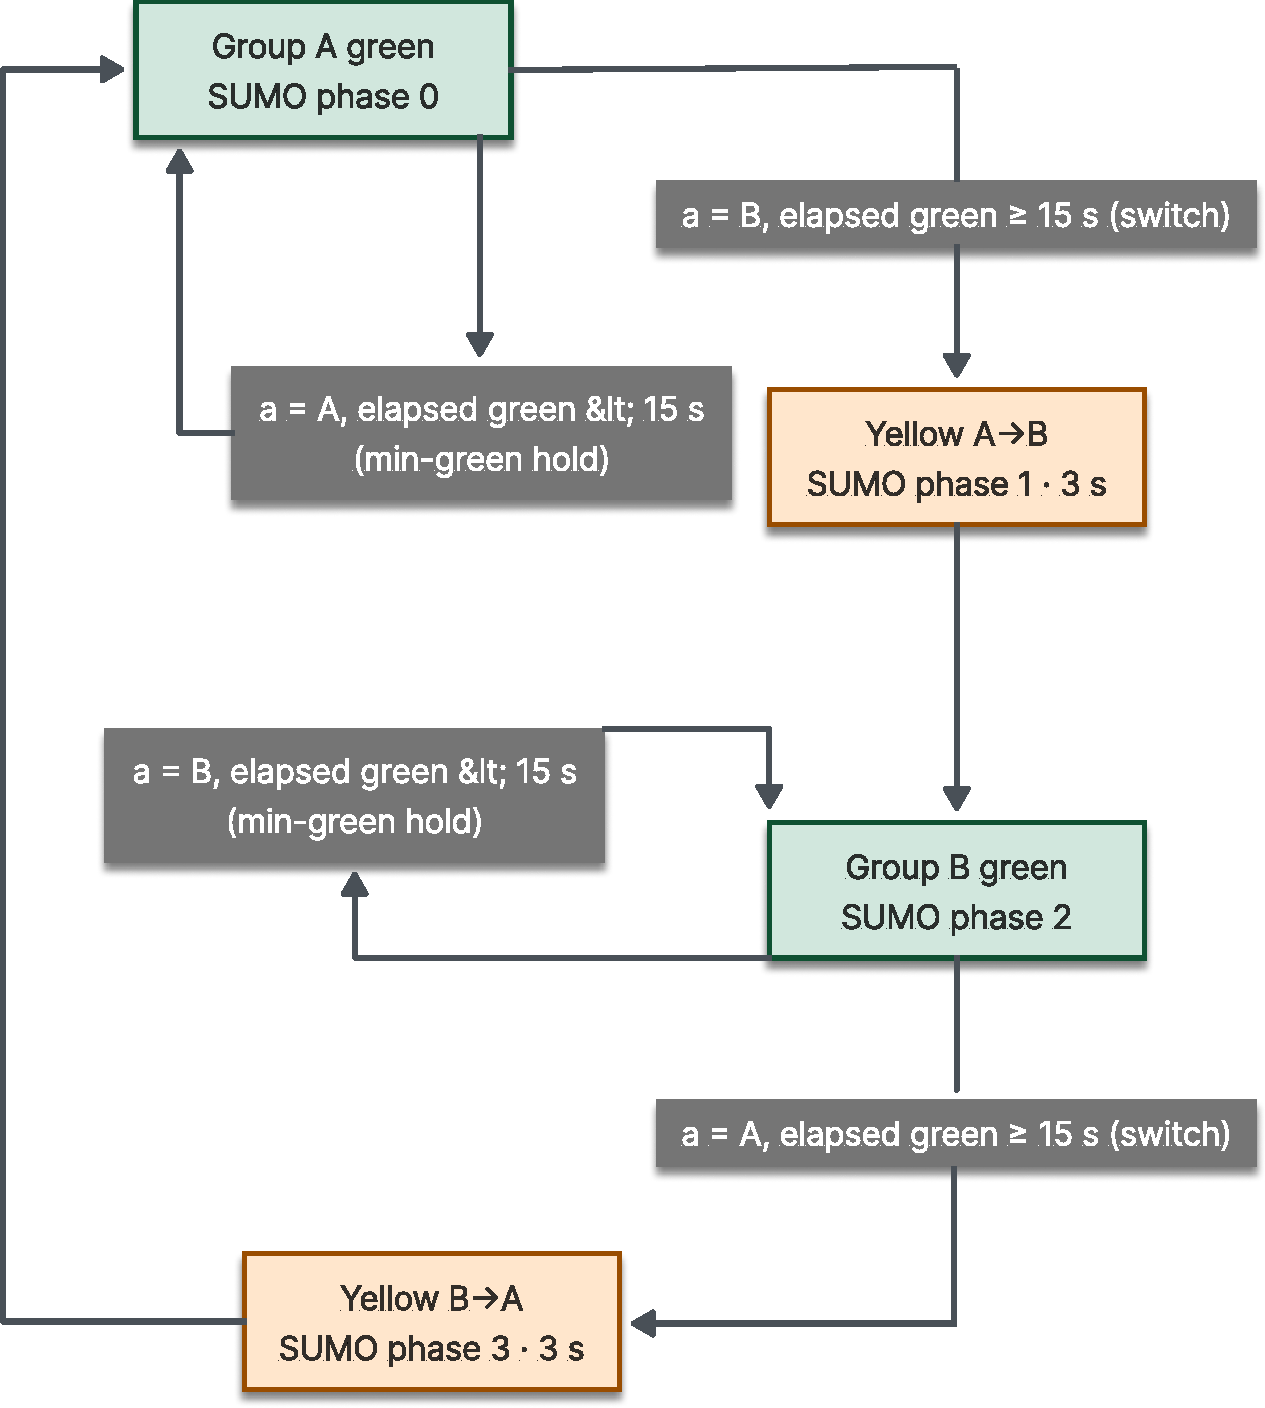
\includegraphics[width=\columnwidth]{assets/figures/fig2.pdf}
   \caption{Two-phase control and environment-enforced timing. At each $5$~s decision
  the binary action selects which non-conflicting group is served. On a switch the
  environment runs a $3$~s yellow clearance and then the new green for the remaining
  $2$~s of the step; the green timer resets to ${\approx}2$~s and accumulates $+5$~s
  per extend, capped at $60$~s. The $15$~s minimum green is a hard constraint, whereas
  the $60$~s maximum only caps the \texttt{green\_timer\_norm} feature and is not a
  forced switch.}
  \label{fig:signal_fsm}
  \vspace{-4mm}
\end{figure}
% NOTE: the Sensing-Noise Model overview (formerly Sec. III-F, \label{sec:noise_model})
% was merged into Sec. VI (Robustness to Sensing Noise) where it is used.
\section{Proposed Methodology}

\subsection{Queue-Centric Vision-Proxy Reward}
\label{sec:reward}
A central contribution of this work is the formulation of a reward function that is
strictly computable from camera-derived proxies, ensuring that the objective optimized
during simulation coincides with the metric available at deployment. The governing design
rule is that every reward term $r^{(k)}_i(t)$ factors through the vision-proxy projection
$\phi(\mathbf{s}_t)$ introduced in Section~\ref{sec:projection}. Unlike prior vision-based reinforcement
learning, which pairs a camera-constrained state with a privileged simulator reward
(typically the exact accumulated delay), no term in the proposed reward reads a privileged
quantity---the accumulated-delay penalty included, which is realized through a
halted-queue proxy. The objective is therefore deployable by construction.

The proposed reward $R_i(t)$ for intersection $i$ is a \emph{queue-centric} objective---a
congestion-minimization core, regularized by a throughput term and a switching term---written
as a weighted sum of six terms:
\begin{equation}
\begin{aligned}
R_i(t)
=&\;
w_q \frac{1}{n_i}\sum_{l=1}^{n_i} q_l^2
+w_p\, p_i(t)
+w_T\, T_i(t) \\
&+
w_s\, \mathbb{1}_{[\text{switch}]}
+w_v \max(\tau-\bar{v},0)
+w_w\, \bar{w}(t),
\end{aligned}
\label{eq:reward}
\end{equation}
where the weights are empirically set to
$w_q=-1.0$,
$w_p=-0.5$,
$w_T=+1.0$,
$w_s=-0.1$,
$w_v=-0.2$,
and
$w_w=-0.3$.
To ensure stable temporal-difference learning, the final scalar is clipped to
$[-2.0,\, +1.5]$. The individual components are detailed below.

These six terms are \emph{not} six orthogonal objectives: four are monotone functions of a
single congestion signal, the per-lane halted-queue fraction $q_l$
(\texttt{effective\_queue\_norm}). The queue penalty applies its $L_2$ norm
($\frac{1}{n_i}\sum_l q_l^2$, the Jensen anti-starvation form below); the accumulated-delay
penalty $\bar{w}(t)$ applies the $L_1$ norm of the \emph{same} vector---no per-vehicle
waiting timer is ever read, so in code it reduces exactly to the mean halted-queue
fraction, supplying a dense low-queue gradient that complements the quadratic term; the
low-speed penalty activates only when the mean approach speed $\bar{v}$ falls below the
threshold $\tau$, targeting stop-and-go congestion; and the phase-imbalance pressure rises
with the same congestion state. The two genuinely distinct regularizers are the local
ROI-exit throughput reward and the phase-switch penalty, the latter suppressing
high-frequency phase flickering. The reward is therefore dense, multi-scale gradient
shaping around a queue-minimization core, and the marginal value of each term
\emph{beyond} the $L_2$ core---rather than an assumption of independence---is what the
ablations of Section~\ref{sec:ablations} quantify.

\paragraph{Anti-starvation queue penalty}
Rather than the linear mean queue over the $n_i$ controlled lanes, the mean of
\emph{squared} queues $\frac{1}{n_i}\sum_{l=1}^{n_i} q_l^2$ is penalized. By Jensen's
inequality this exceeds the squared mean by exactly the per-lane queue variance, so the
quadratic form penalizes spatial imbalance at equal total demand and thereby discourages
the starvation of minor approaches.

\paragraph{Phase-imbalance pressure}
A signed \emph{phase-imbalance} term $p_i(t) \in [-1, 1]$ measures the queue delta between the
two fixed phase groups at the \emph{same} junction, partitioned by the currently red and green
movements:
\begin{equation}
p_i(t) = \frac{1}{n_i} \left( \sum_{l \in \text{red}} q_l - \sum_{l \in \text{green}} q_l \right).
\label{eq:pressure}
\end{equation}
This is an \emph{intra-junction} demand-imbalance gradient and is explicitly \emph{not} the
upstream--downstream network pressure of classical max-pressure
control~\cite{varaiya2013_maxpressure}; accordingly we do not claim the throughput-optimality
guarantee of max-pressure routing, and---compounded by per-lane normalization and value
clipping---the term functions as a highly reactive local heuristic rather than an optimal
routing policy. In contrast to a one-sided $\max(p, 0)$ surrogate, which provides zero gradient
whenever the active allocation is already correct, the signed form supplies a continuous
gradient that rewards serving the more congested group and penalizes serving the emptier one.

A naming subtlety: the reward pressure $p_i(t)$ is \emph{signal-relative}---evaluated
over the dynamic red/green partition induced by the active phase---whereas the
observation feature $\mathrm{pressure\_norm}$ of Section~\ref{sec:obs_space} is
\emph{geometry-relative}, encoding the static group-mean imbalance over the fixed groups
$A, B$. The phase one-hot identifies which fixed group holds green and
$\bar{q}_A - \bar{q}_B = 2\,\mathrm{pressure\_norm} - 1$, so the reward pressure is an
affine, phase-determined transform of observed quantities (exact up to approach
aggregation, equal-group scaling, and boundary saturation): the actor observes the
information its pressure reward optimizes.

\paragraph{Local ROI-exit throughput}
The agent is rewarded for vehicles actively clearing the intersection. The throughput term
is defined as
\begin{equation}
T_i(t) = \mathrm{clip}\!\left(\frac{1}{\kappa}\sum_{l \in L_i}\bigl|\, \text{prev\_ids}(l) \setminus \text{cur\_ids}(l)\, \bigr|,\; 0,\; 1\right),
\label{eq:throughput}
\end{equation}
with normalizing capacity $\kappa = 20$ and $L_i$ the set of lanes controlled by agent $i$.
Crucially, the simulator computation---the set difference of per-lane vehicle identities
between consecutive steps in SUMO~\cite{lopez2018_sumo}---is \emph{semantically identical}
to the deployable measurement of track identities terminating at the boundary of a
ByteTrack~\cite{zhang2022_bytetrack} region of interest (ROI). The reward signal is thus a
deployable metric in itself, incurring no domain shift. Because an exit is registered for
any identity present at the previous step and absent at the current one, lateral lane
changes (frequent under the sublane model) and the rare SUMO teleport are also counted as
exits; this is a bounded source of measurement noise that the deployable ByteTrack ROI-exit
counter shares identically, and therefore introduces no train/deploy discrepancy.

\subsection{MAPPO Architecture and Optimization}
\begin{figure*}[!t]
\centering
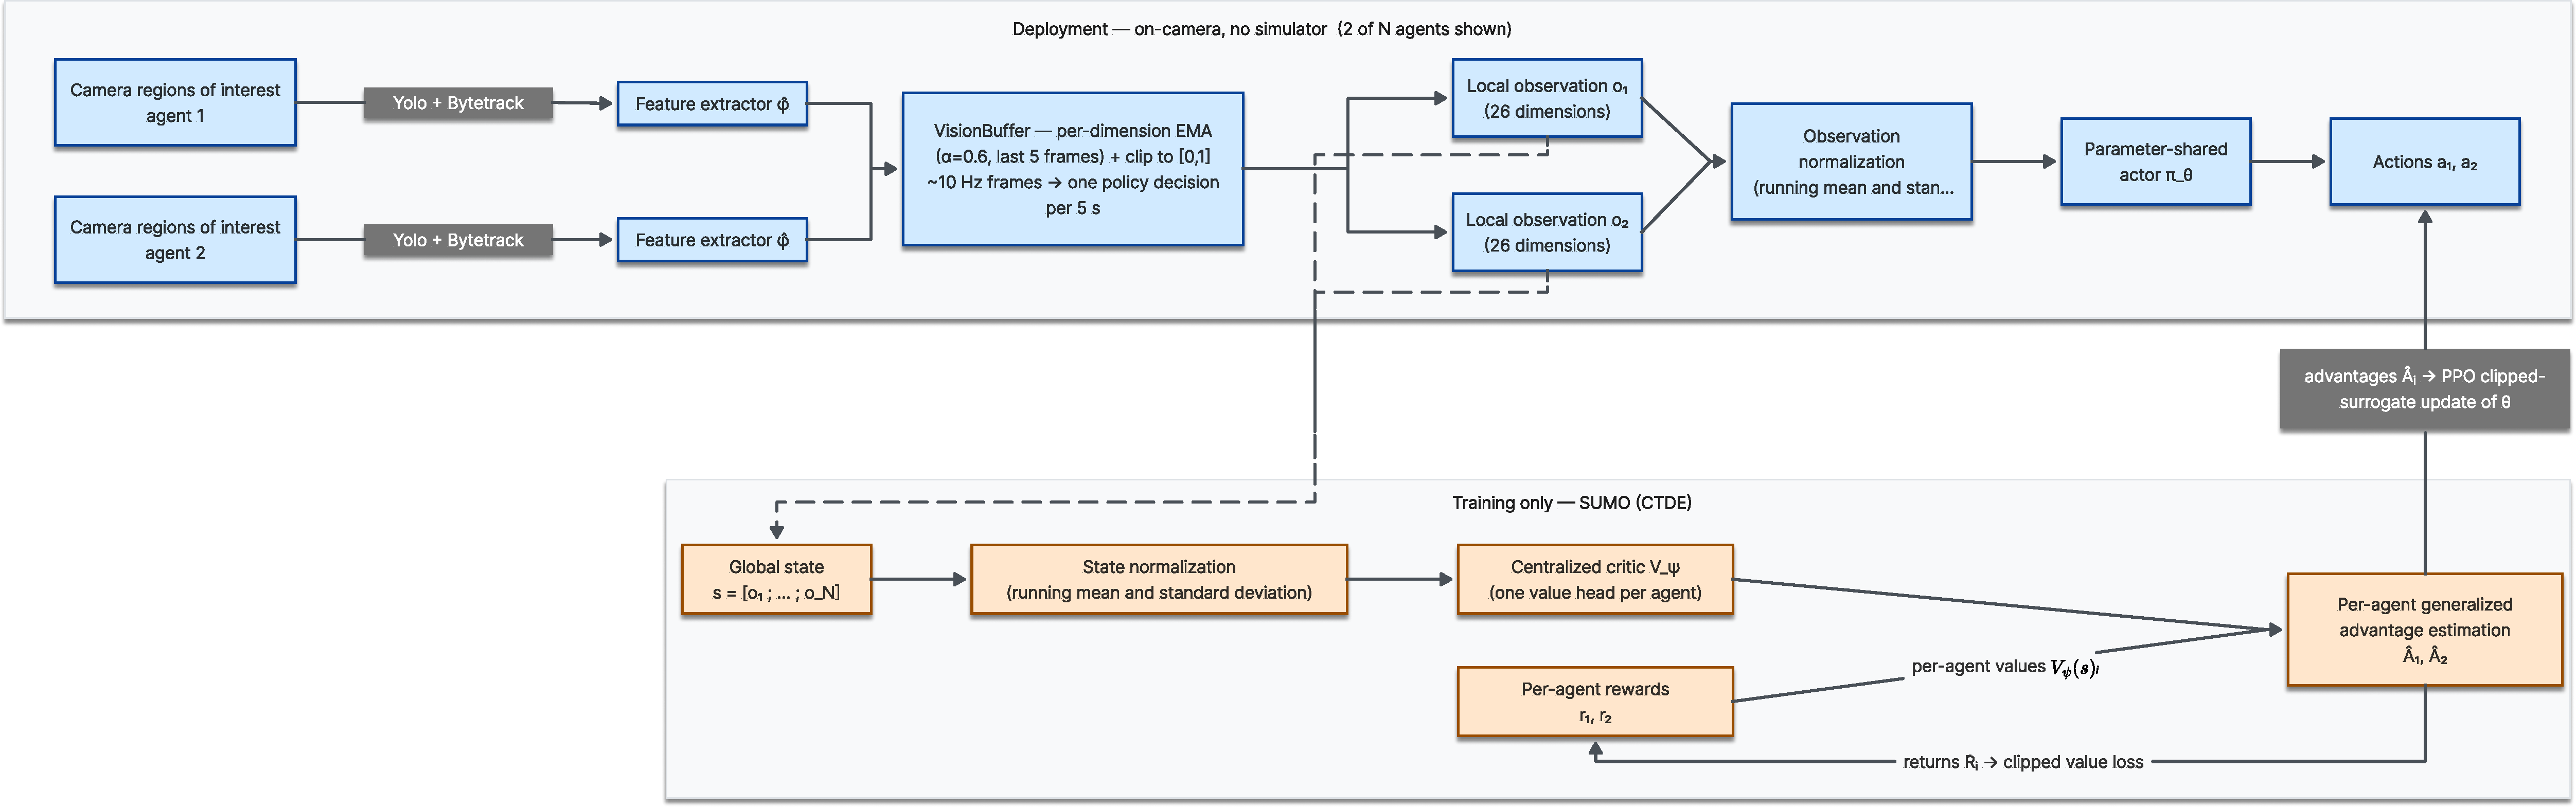
\includegraphics[width=\textwidth]{assets/figures/system_architecture.pdf}
\caption{Overall architecture of the proposed camera-observable multi-agent control
framework. Solid paths denote the on-camera deployment data flow (no simulator): per-agent
regions of interest are processed by YOLOv11 and ByteTrack, smoothed by a per-dimension
VisionBuffer (EMA, $\alpha=0.6$), normalized by the serialized Welford statistics, and
mapped to discrete phase actions by the parameter-shared actor $\pi_\theta$. Dashed paths
denote the training-only centralized multi-head critic and the per-agent GAE
estimator, neither of which is deployed.}
\label{fig:architecture}
\vspace{-4mm}
\end{figure*}

To optimize the multi-agent control policy, Multi-Agent Proximal Policy Optimization
(MAPPO)~\cite{yu2022_mappo} is adopted---a standard instance of the Centralized Training
with Decentralized Execution (CTDE) paradigm for the Dec-POMDP~\cite{oliehoek2016_decpomdp}
formalized in Section~\ref{sec:problem}. It is emphasized that the reinforcement-learning architecture
itself is standard and is not claimed as a methodological contribution; rather, it serves
as the vehicle through which the proposed camera-constrained state and vision-proxy reward
are evaluated.

The framework comprises a parameter-shared actor $\pi_\theta(a_{i,t}\,|\,\mathbf{o}_{i,t})$
that operates on the $26$-dimensional local proxy observation, yielding homogeneous control
behavior across intersections and facilitating zero-shot transfer to unseen topologies.
During training, a centralized critic $V_\psi(\mathbf{s}_t)$ ingests the concatenated global
proxy state. To preserve agent-specific reward shaping, the critic employs a multi-head
architecture that emits one value estimate per agent; this distinguishes the method from
the independent-critic IPPO~\cite{dewitt2020_ippo} baseline, in which each agent estimates
value from its local observation alone. Coordination in this design is achieved
\emph{solely} through the centralized critic: the per-agent rewards $r_{i,t}$ are strictly
local---each agent is credited only for the queues, phase imbalance, and ROI exits on its own
approaches, matching the deployment camera's field of view---so no inter-agent term appears in
the reward itself. Cross-intersection credit assignment enters only via the concatenated global
state ingested by the critic during centralized training and is absent at decentralized
execution, consistent both with the CTDE paradigm and with the camera-only constraint on the
deployed actor. Advantages $\hat{A}_{i,t}$ are computed via per-agent Generalized Advantage Estimation
(GAE)~\cite{schulman2016_gae} on the decentralized reward streams and standardized across all
agents within the batch. The actor and critic are then optimized using the standard PPO clipped
surrogate objective and a clipped multi-head value loss, respectively~\cite{schulman2017_ppo},
with early stopping triggered if the approximate KL divergence exceeds $1.5\times$ the target.

To bridge the residual normalization gap between training and deployment, the observation
running mean and variance are tracked online by Welford's algorithm~\cite{welford1962} and
serialized directly into the deployment checkpoint alongside the actor weights. Test-time
inputs $\mathbf{o}_{i,t}$ are therefore normalized with statistics identical to those seen
during training, without any dependence on live estimation.
\section{Experimental Setup}
\label{sec:experimental_setup}

\subsection{Simulation Environment and Mixed-Traffic Calibration}
\label{sec:sim_env}
All experiments are conducted in SUMO~v1.12.0~\cite{lopez2018_sumo}, configured with
the sub-lane model at a lateral resolution of $0.4$~m. This choice is deliberate
rather than cosmetic: in motorcycle-dominant traffic the conventional one-vehicle-per-lane
abstraction is invalid, as powered two-wheelers continuously filter laterally and form
wide, deformable clusters that conventional car-following models cannot reproduce. The
sub-lane resolution restores the lateral degrees of freedom required to capture this
filtering behaviour, consistent with microscopic observations of motorcycle dynamics under
Vietnamese mixed-traffic conditions~\cite{vn_roundabout}.

The vehicle composition is a central calibration target. The motorcycle count share is set
to $73\%$, anchored to the $72.6\%$ motorcycle mode share reported for
Ngoc~\emph{et~al.}~\cite{ngoc2021_fivecities}; the remaining demand is allocated to
passenger cars ($17\%$), trucks ($7\%$), and buses ($3\%$) by vehicle class.
Ngoc~\emph{et~al.}~\cite{ngoc2021_fivecities} also reports motorcycle shares of $\approx 80$--$89\%$ for Hai~Phong, Da~Nang, Ho~Chi~Minh~City, and
Can~Tho, a range deliberately bracketed by the composition sweep of
Section~\ref{sec:generalization}. We distinguish count share from traffic \emph{load}: at a motorcycle
passenger-car-unit (PCU) equivalence of $\approx 0.29$~\cite{cao_sano_hanoi},
a $73\%$ motorcycle count corresponds to only about one-third of the total PCU-based load,
with the exact fraction depending on the heavy-vehicle PCU values. Accordingly, count share
is used when reasoning about lateral filtering, whereas PCU is used for capacity
arguments. To reproduce realistic motorcycle swarming, the sub-lane parameters are set to
\texttt{latAlignment=arbitrary} with a minimum lateral gap \texttt{minGapLat},
which allows roughly three to four motorcycles to share a standard $3.2$~m urban lane
alongside a passenger car.

Under this calibration, a queue-discharge experiment yields a raw per-lane discharge of
approximately $2450$~veh/h---well above a conventional car-lane saturation flow because
motorcycles filter and discharge several abreast within a single lane. At the calibrated
$73\%$ motorcycle share this corresponds to roughly $1500$~PCU/h per lane, characteristic of
the mixed-flow regime documented for Hanoi~\cite{cao_sano_hanoi}. As regional compositions vary, the $73\%$ value is treated
as a representative anchor rather than a universal constant, and the policy's robustness to
compositional shift is defended explicitly through the systematic motorcycle sweep
($\{50\%, 73\%, 90\%\}$) of Section~\ref{sec:generalization}.

\subsubsection{Signal-Timing Bounds}
The minimum green time is fixed at $15$~s (three decision intervals).
This ensures that an activated phase discharges a meaningful platoon and suppresses the high-frequency
phase flickering that otherwise traps wide motorcycle clusters within the intersection. The
maximum green time is fixed at $60$~s. This value is justified by a simulation-based
design-selection pilot on the $16$-junction N3 grid (seed~$42$, $100$k training steps),
evaluated on held-out demand. As reported in Table~\ref{tab:maxgreen_pilot}, the $60$~s
bound dominates a relaxed $90$~s bound across all primary metrics; in particular, the
$90$~s bound severely degrades the $95$th-percentile (P95) waiting time
(the selected $60$~s bound is $24.7\%$ lower), because excessively long green phases starve cross-phase
movements, conflicting directly with the anti-starvation objective of the reward
(Section~\ref{sec:reward}). The bounds are therefore adopted as a structural
choice applied uniformly to every learned and heuristic controller. We note that the
maximum green time additionally sets the scale of the \texttt{green\_timer\_norm} feature
($\text{timer}/\text{max\_green}$); it is thus a coupled observation/model parameter
prior to training and held identical across all arms, with the SUMO-actuated controller's
\texttt{maxDur} matched to $60$~s for fairness.

\begin{table}[t]
  \centering
  \caption{Maximum-green selection pilot (N3 grid, seed~$42$, $100$k steps, held-out
  evaluation). Lower is better; the selected bound is in bold. Evaluation is based on an early
  $100$k-step convergence pilot used to structurally set the signal-timing constraints prior
  to full training, not on the converged policy.}
  \label{tab:maxgreen_pilot}
  \vspace{-4mm}
  \begin{tabular}{lccc}
    \toprule
    \textbf{Max-green} & \textbf{Travel time (s)} & \textbf{Waiting (s)} & \textbf{P95 waiting (s)}\\
    \midrule
    \textbf{$60$~s (selected)} & \textbf{311.1} & \textbf{135.8} & \textbf{504}\\
    $90$~s                     & 367.0          & 173.6          & 669\\
    \midrule
    $\Delta$ ($60$ vs.\ $90$)  & $-15.2\%$      & $-21.8\%$      & $-24.7\%$\\
    \bottomrule
  \end{tabular}
\end{table}

\subsection{Networks and Demand}
\label{sec:networks}
The framework is evaluated on two synthetic but structurally sound topologies: a
signalized corridor (denoted N2; $1 \times 5$ junctions) and a signalized grid
(denoted N3; $4 \times 4$ junctions). All intersections are four-way with two lanes per approach. The two scales
jointly probe both arterial coordination (the corridor) and network-level interaction under
many simultaneously learning agents (the grid).

To stress-test the controllers under non-stationary load rather than a single operating
point, vehicle insertions over the $5400$~s episode are drawn from an inhomogeneous Poisson
process following a time-varying trapezoidal profile. The profile ramps from an off-peak lull
to a sustained demand peak, eases to an intermediate plateau, and tapers back, exercising the
controllers across loading, saturation, and unloading regimes. The exact mathematical
formulation and rate parameters are provided in Appendix~\ref{app:demand}.
\begin{figure}[t]
    \centering
    \begin{subfigure}{\columnwidth}
        \centering
        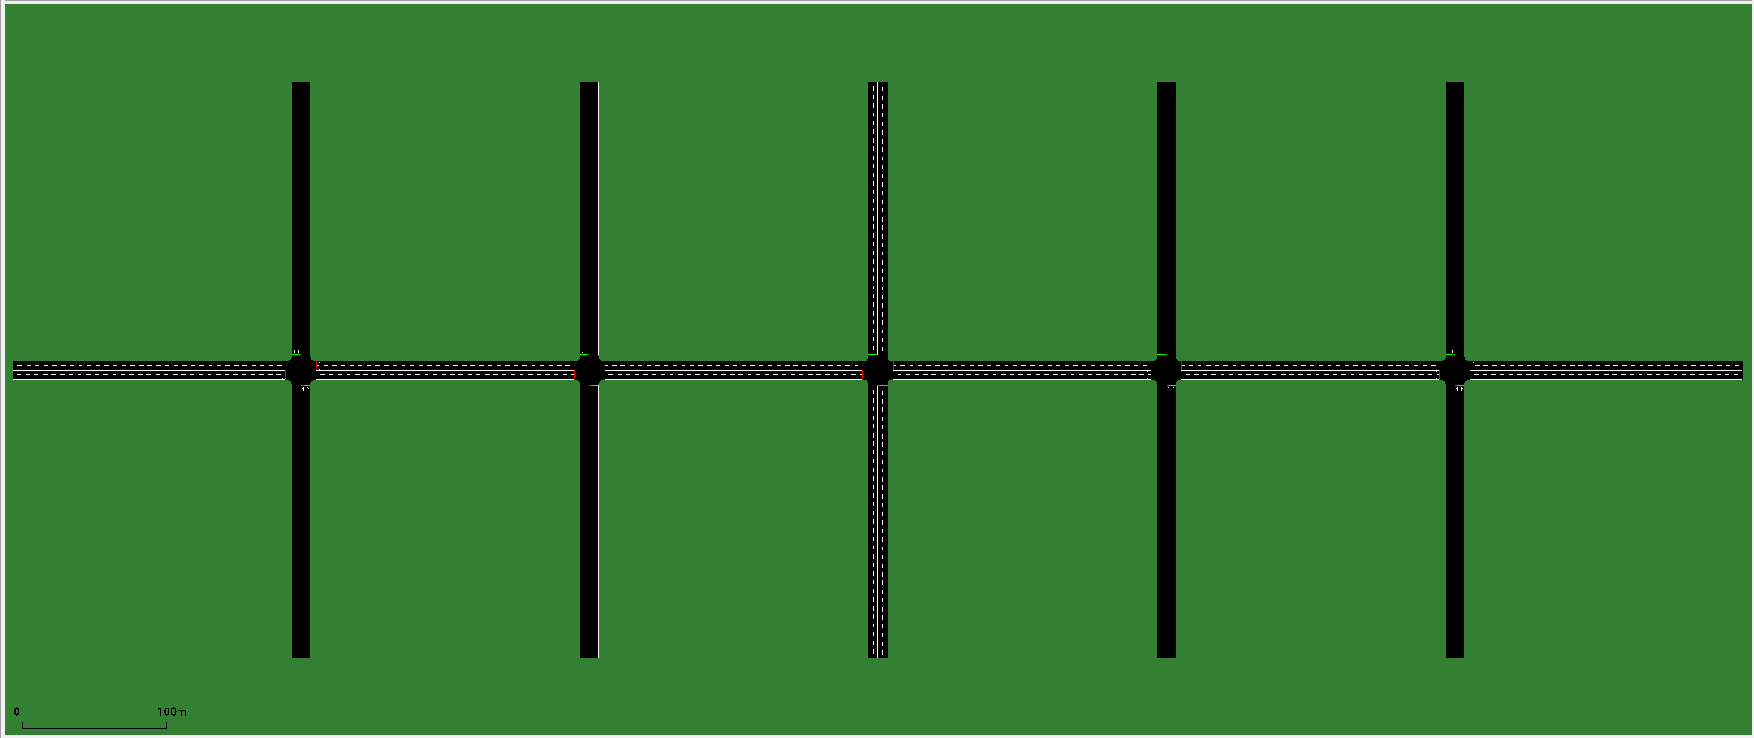
\includegraphics[width=\columnwidth]{assets/figures/n2_sumo.pdf}
        \caption{N2 corridor ($1\times5$, 5 intersections).}
        \label{fig:net_n2}
    \end{subfigure}
    \vspace{2mm}
    \begin{subfigure}{\columnwidth}
        \centering
        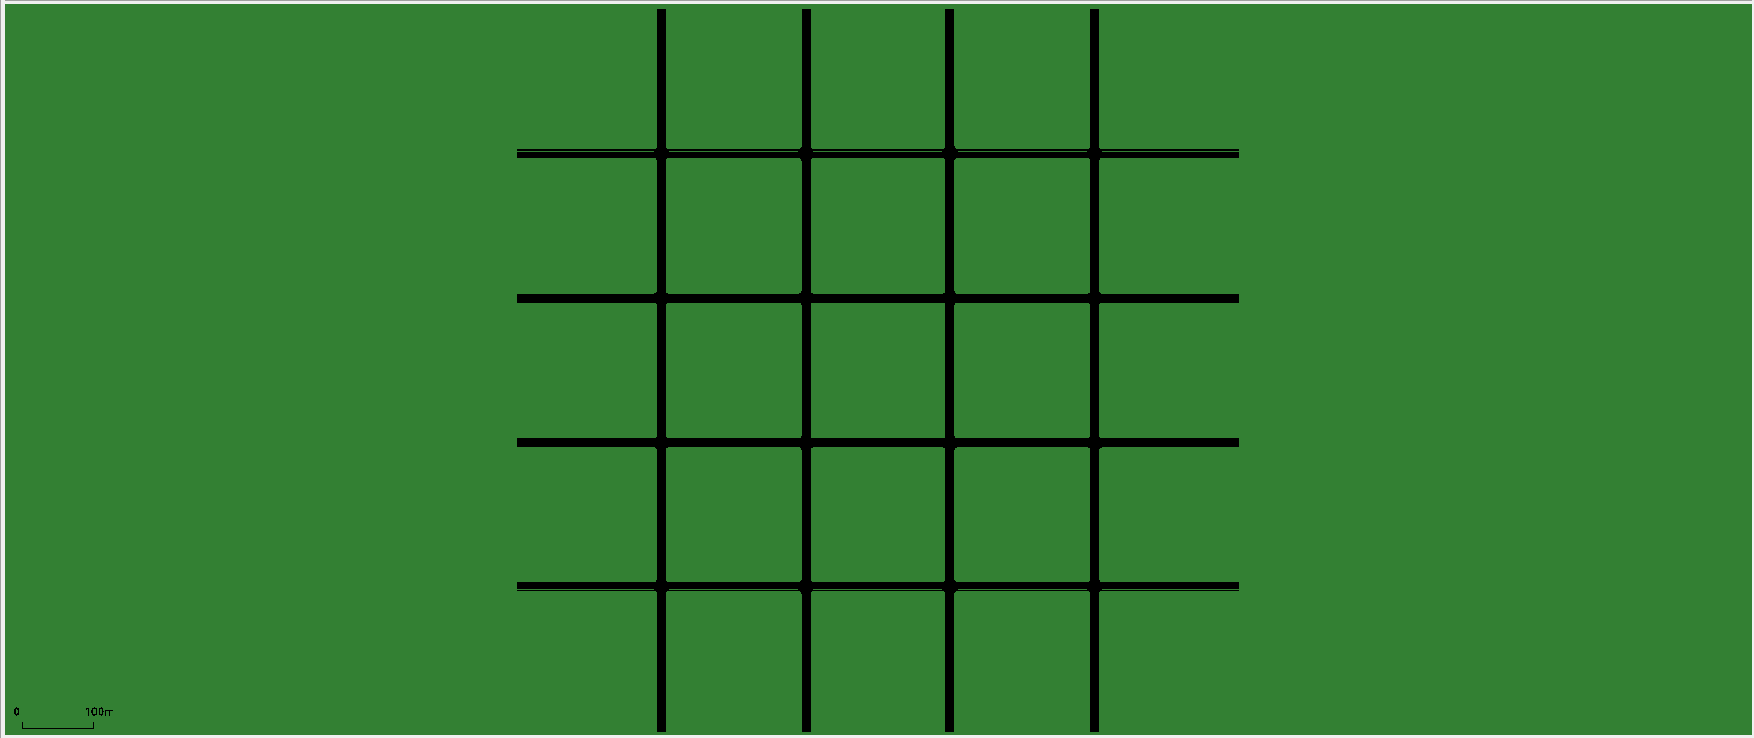
\includegraphics[width=\columnwidth]{assets/figures/n3_sumo.pdf}
        \caption{N3 grid ($4\times4$, 16 intersections).}
        \label{fig:net_n3}
    \end{subfigure}
    \caption{SUMO evaluation networks. All intersections are four-way with two lanes per approach; each intersection is controlled by one decentralized MAPPO agent.}
    \label{fig:networks}
    \vspace{-4mm}
\end{figure}
\subsection{Baselines}
\label{sec:baselines}
The proposed MAPPO controller is benchmarked against a spectrum of strong, non-strawman
baselines. To ensure a fair comparison, every heuristic is restricted to the same phase
groups, decision interval, and timing constraints as the learned policy.
\begin{itemize}
  \item \emph{Webster fixed-time}~\cite{webster1958}: an analytically derived fixed-time
        plan computed from PCU-weighted measured flows, with cycle length
        $C = (1.5L + 5)/(1 - Y)$ clamped to $[40, 120]$~s and proportional green splits.
        This provides a competitive classical baseline rather than a degenerate fixed-time
        plan. To ensure a strict and fair comparison, Webster's saturation flow is explicitly
        calibrated to the network's measured mixed-traffic sublane capacity
        ($\approx 1500$~PCU/h/lane), preventing artificial performance degradation that would
        occur if standard car-only saturation flows were assumed.
  \item \emph{SUMO-actuated}: the gap-based actuation controller native to
        SUMO~\cite{lopez2018_sumo}, configured with \texttt{minDur}~$=15$~s and
        \texttt{maxDur}~$=60$~s to match the learned controllers exactly.
  \item \emph{Max-Pressure}~\cite{varaiya2013_maxpressure}: a greedy pressure-based
        heuristic that consumes the identical observation pipeline and phase groups as the
        RL agents and grants right-of-way to the phase of highest pressure.
  \item \emph{IPPO}~\cite{dewitt2020_ippo}: an ablative learned baseline with an identical
        actor architecture and training budget but with independent per-agent critics
        conditioned solely on the local $26$-dimensional observation.
        This isolates the contribution of centralized training with decentralized execution.
  \item \emph{MAPPO-privileged (upper bound)}: the identical MAPPO~\cite{yu2022_mappo}
        algorithm whose observation is augmented to a $38$-dimensional vector incorporating
        exact, non-camera-observable simulator quantities (exact halting counts,
        waiting times, and total vehicle counts). The reward is held identical to the proxy
        arm and only the state visibility differs, so the gap between this arm and the proxy
        policy directly quantifies the \emph{information-restriction cost} of
        Section~\ref{sec:restriction_cost}.
\end{itemize}

\subsection{Metrics and Statistical Protocol}
\label{sec:metrics}
Performance is quantified by two primary metrics extracted from SUMO's \texttt{tripinfo}
output: mean travel time and mean waiting time. Secondary metrics comprise the P95 waiting
time (which captures starvation events masked by the mean), the throughput ratio, the mean
vehicle speed, and the number of phase switches per episode. Environmental indicators
(CO\textsubscript{2} emissions and fuel consumption, computed via the HBEFA-based emission
model~\cite{krajzewicz2015_emissions}) are evaluated post hoc and are never exposed to the
agent reward.

To ensure statistical rigour, each method is trained with five independent seeds
($42, 123, 456, 789, 1337$) and evaluated on ten held-out demand route-seeds per scenario.
All tabular results report the mean across training seeds together with a $95\%$ confidence
interval. Statistical significance is assessed against the strongest baseline using a
two-sided Mann--Whitney $U$ test~\cite{mann1947_mwu}, with $p$-values corrected for multiple
comparisons across scenarios by the Holm--Bonferroni procedure~\cite{holm1979}.
Effect size is reported through Cohen's~$d$~\cite{cohen1988} to guard against
statistically significant but negligible differences.

\subsection{Training Configuration and Reproducibility}
\label{sec:training}
Each model is trained to a fixed budget of $5 \times 10^{5}$ environment steps, a
horizon established by convergence pilots. Observation statistics are normalized by
Welford's algorithm~\cite{welford1962} and serialized into the checkpoint, so that
evaluation and deployment apply identical normalization without recompilation. The complete
set of MAPPO training hyperparameters---including PPO clip ratios, GAE discount factors, and
learning rates---is detailed in Appendix~\ref{app:hyperparams}.

To guarantee end-to-end reproducibility, the full codebase, trained checkpoints,
demand generators (\texttt{.rou.xml}), phase-group derivations, and evaluation scripts are
released publicly at \mbox{[REPOSITORY~URL]} under a tagged commit. The precise observation
and reward schema version is stamped into every run configuration, ensuring that all
results are traceable to an exact environment specification.

% [Hyperparameter table relocated to Appendix~\ref{app:hyperparams} (sec9_appendices.tex)]

\section{Experimental Results}
\label{sec:results}

\subsection{Quantitative Performance Comparison}
\label{sec:res_quantitative}
Analysis of throughput, average queue lengths, and waiting times against baseline heuristics goes here.

\subsection{Information-Restriction Cost: Proxy vs.\ Privileged}
\label{sec:restriction_cost}
The performance gap between the camera-proxy policy and the privileged-observation upper bound (identical reward, $38$-dimensional state) goes here.

\subsection{Generalization: OOD Demand and Composition Sweep}
\label{sec:generalization}
Out-of-distribution demand (low/medium/high/asymmetric) and the motorcycle-share sweep ($\{50, 73, 90\}\%$) go here.

\subsection{Robustness Analysis under Sensing Noise}
\label{sec:robustness_noise}
Evaluation of the proxy policy's degradation under the calibrated camera-noise sweep ($\{0, 0.5, 1, 2\}\times$), including Table~\ref{tab:noise_params}, goes here.

\subsection{Ablation Studies}
\label{sec:ablations}
Retrained reward-preset and observation ablations (C1 state elements, C2 reward components) go here.

\section{Discussion and Limitations}
\label{sec:discussion}

The central question posed by this work is not whether multi-agent reinforcement learning
can control traffic signals---this is well established---but how much of that capability
survives when the policy is denied every privileged simulator quantity and restricted to
signals a roadside camera can actually compute. The experiments answer this quantitatively.
The information-restriction cost, defined as the performance gap between the proxy policy and
the privileged upper bound under identical pristine features (Section~\ref{sec:restriction_cost}),
is only $\RestrictionCost\%$ in mean travel time, while the proxy policy itself improves on the strongest
classical baseline by $\ImproveStrongest\%$. The interpretation is direct: for the signal-timing objective,
the camera-observable feature set retains the overwhelming majority of information, and the
residual loss from discarding exact per-vehicle delays and network-wide counts is small
relative to the gains from learning itself. This isolates a result that prior camera-state RL
leaves implicit, because those methods constrain the observation while continuing to train on
a privileged reward~\cite{azfar2025_cosim,dai2022_worldmodels}; here the reward is itself
camera-computable, so the reported cost reflects a genuinely deployable controller rather than
a partially privileged one.

The mechanism behind this performance is illuminated by the ablations
(Section~\ref{sec:ablations}). The two reward components designed against starvation---the
mean-of-squared-queue penalty and the signed phase-imbalance term---contribute disproportionately to
the tail-latency metric: removing either inflates the P95 waiting time far more than the mean,
confirming that the quadratic penalty and the directional phase-imbalance signal act precisely where
a linear queue average and a one-sided pressure surrogate~\cite{varaiya2013_maxpressure,
wei2019_presslight} are blind. The advantage of centralized training over the independent-critic
variant~\cite{dewitt2020_ippo} further indicates that the observed gains are not merely the
product of a richer state, but of coordinated credit assignment across multiple intersections
under shared, non-stationary demand.

These findings should be read as closing an \emph{observation} gap, which is distinct from,
and complementary to, the \emph{dynamics} gap that dominates sim-to-real transfer in robotics
and in prior transfer-oriented TSC~\cite{peng2018_dynrand,zhao2020_sim2real_survey,
da2024_promptgat}. The graceful degradation observed across the $\{0\times,0.5\times,1\times,2\times\}$
sensing-noise envelope (Section~\ref{sec:robustness_noise}) shows that the policy does not rely
on brittle, high-precision feature recovery: performance declines smoothly rather than
collapsing as perception error grows, and the relative ordering against the heuristic baselines
is preserved throughout. We emphasize that this is evidence about the policy's tolerance to
bounded perception error under a documented-basis noise model, not a claim of guaranteed field
transfer; the latter requires the dynamics gap to be addressed in tandem and is the subject of
the companion study.

From a practitioner's standpoint, the practical implication is that adaptive, learned signal
control need not wait for instrumented intersections or privileged feedback channels. A single
camera and a legacy two-phase controller---the prevailing hardware in many developing
metropolises---are sufficient to host the policy, since every quantity required at inference
is derived from detection and tracking alone. This lowers the deployment barrier from a
sensing-infrastructure problem to a calibration-and-integration problem.

\noindent\textbf{Limitations and future work.}
While this study isolates the information-restriction cost of camera-computable control,
several limitations remain. First, the evaluation employs a two-phase logic without protected
turns, matching legacy hardware but limiting international generality. Second, the 1D effective
queue is a scalar proxy for 2D sublane flow, and the local throughput reward introduces a minor
theoretical risk of downstream spillback (greedy flushing) that the central critic only
partially mitigates. Finally, the findings establish the robustness boundary in simulation;
bridging the physical dynamics gap with measured feature-recovery calibration is left to the
companion field deployment.

\section{Conclusion}
\label{sec:conclusion}

This paper addressed the persistent observation gap in reinforcement-learning-based traffic
signal control by imposing a single, strict constraint throughout the formulation: both the
state and the reward must be computable from a roadside camera alone. Concretely, a
$26$-dimensional per-approach proxy observation was paired with a fully camera-computable,
queue-centric vision-proxy reward, so that the objective optimized in simulation coincides with the
quantity available at deployment, with no privileged simulator signal entering either the
policy input or the training target. On a sixteen-junction grid under non-stationary,
motorcycle-dominant demand, the resulting MAPPO controller improved mean travel time over
every camera-deployable baseline---by $\ImproveStrongest\%$ against the strongest of
them---while remaining statistically indistinguishable from a loop-instrumented gap-actuated
reference, and the gap to a privileged upper bound---the information-restriction cost---was
only $\RestrictionCost\%$. On a single-axis arterial corridor, by contrast, classical
progression control remained superior: the reversal is structural---queue-centric objectives
encode no progression incentive---and delineates the topology regime in which learned
camera-only control repays its complexity. The policy further degraded
gracefully across a $\{0\text{--}2\times\}$ sensing-noise envelope, retaining its advantage over
the heuristic baselines throughout, which indicates that the approach does not depend on
high-precision feature recovery.

Taken together, these results establish that the privileged-data dependency long assumed by
RL-based signal control is largely unnecessary for the timing objective itself: the
camera-observable feature set is shown, in simulation, to retain the overwhelming majority of
the task-relevant information. For practitioners in developing metropolises, this lowers the
barrier to adaptive control from a sensing-infrastructure problem to a calibration-and-integration
one, since a single overhead camera and a legacy two-phase controller suffice to host the policy.
Future work will extend the action space to multi-phase ring-barrier logic with protected
turns, will augment the vision-proxy objective with explicit, camera-computable progression
incentives for arterial deployment, and will close the physical control loop in the companion
field study, where the dynamics gap and a measured perception calibration complement the
observation gap quantified here.

% \appendices
% \section{Hyperparameters and Network Details}
\label{app:hyperparams}
Table~\ref{tab:hyperparams} lists the complete MAPPO training hyperparameters used for every
learned arm. The IPPO baseline and the privileged upper bound share this identical schedule,
differing only in the critic structure (independent per-agent critics) and the observation
dimension (an augmented $38$-dimensional state), respectively.

\begin{table}[h]
\centering
\caption{MAPPO training hyperparameters.}
\label{tab:hyperparams}
\begin{tabular}{lc}
\toprule
\textbf{Hyperparameter} & \textbf{Value} \\
\midrule
Discount factor ($\gamma$)      & $0.99$ \\
GAE parameter ($\lambda$)       & $0.95$ \\
PPO clip ratio ($\epsilon$)     & $0.2$ \\
Target KL divergence            & $0.015$ \\
Learning rate                   & $3 \times 10^{-4}$ (linear decay) \\
Rollout horizon                 & $128$ steps \\
Minibatch size                  & $256$ \\
Optimization epochs             & $10$ \\
Total environment steps         & $5 \times 10^{5}$ \\
\bottomrule
\end{tabular}
\end{table}

\section{Time-Varying Demand Profile}
\label{app:demand}
The per-episode demand follows a time-varying rate $\lambda(t)$ of duration $5400$~s, realized
as an inhomogeneous Poisson process whose rate is the piecewise-linear (trapezoidal) function
\begin{equation}
  \lambda(t) = \mathrm{PWL}\!\left(t;\, \mathbf{t}_k,\, \boldsymbol{\lambda}_k\right),
  \label{eq:demand}
\end{equation}
linearly interpolated between the knot times $t_1=0$, $t_2=900$, $t_3=1500$, $t_4=3000$,
$t_5=3600$, $t_6=4800$, and $t_7=5400$~s, with corresponding base rates $\lambda_1=0.4$,
$\lambda_2=0.4$, $\lambda_3=1.67$, $\lambda_4=1.67$, $\lambda_5=0.83$, $\lambda_6=0.83$, and
$\lambda_7=0.4$~veh/s, scaled proportionally to the number of network entries. The profile thus
advances from an off-peak lull, ramps to a sustained demand peak over $1500$--$3000$~s, eases to
an intermediate plateau over $3600$--$4800$~s, and finally tapers back to off-peak, exercising
the controllers across loading, saturation, and unloading regimes within a single episode.
\textbf{}

\section*{Acknowledgment}
The authors would like to thank the Institute of Intelligent and Interactive Technologies (3IT), University of Economics Ho Chi Minh City (UEH), for providing the computational resources and infrastructure that supported this research.

\ifCLASSOPTIONcaptionsoff
  \newpage
\fi

\nocite{*}
\bibliographystyle{IEEEtran}
\bibliography{references} 


\begin{IEEEbiography}[{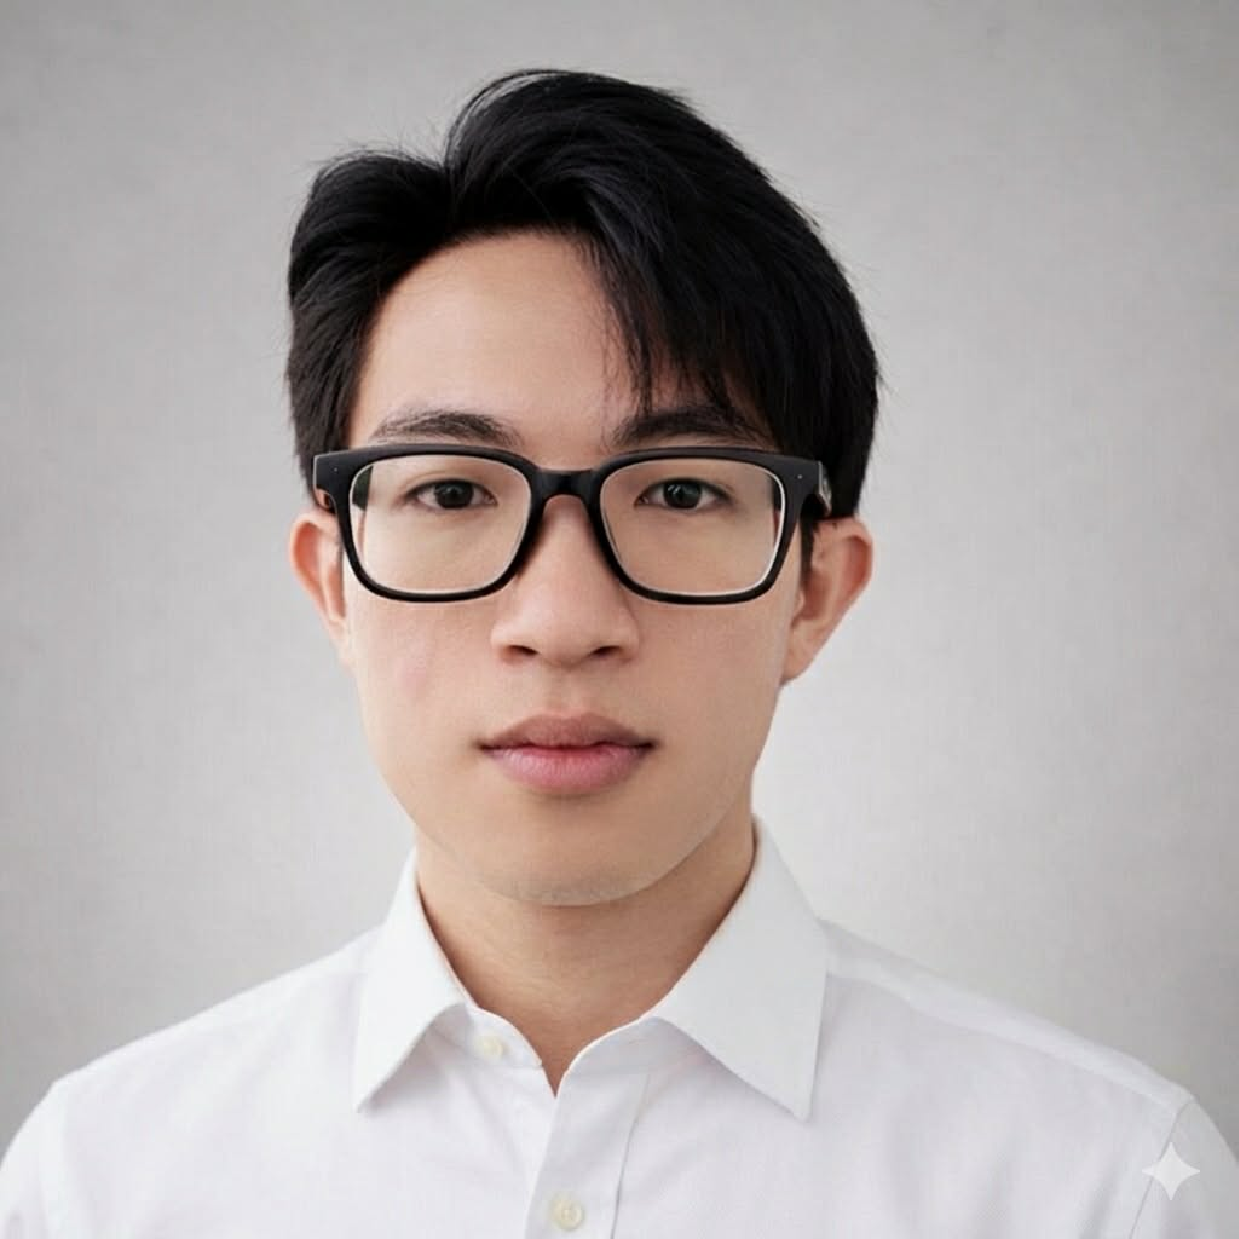
\includegraphics[width=1in,height=1.25in,clip,keepaspectratio]{tronghia.pdf}}]{Le Trong Nghia}
received his high school diploma in 2024. He is currently pursuing his B.S. degree in Robotics and Artificial Intelligence at the Institute of Intelligent and Interactive Technologies, University of Economics Ho Chi Minh City (UEH), Ho Chi Minh City, Vietnam. His current research interests include deep reinforcement learning, multi-agent systems, intelligent transportation systems (ITS), and computer vision.
\end{IEEEbiography}
\begin{IEEEbiography}[{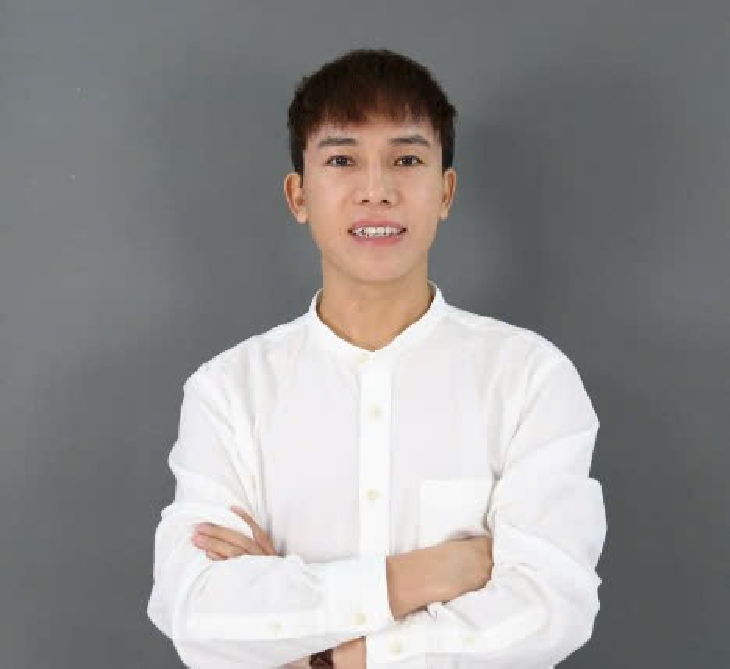
\includegraphics[width=1in,height=1.25in,clip,keepaspectratio]{ntbao.pdf}}]{Nguyen Thien Bao}
(Member, IEEE) received his Ph.D. degree in Computer Science. He is currently a Lecturer and Researcher with the Institute of Intelligent and Interactive Technologies, University of Economics Ho Chi Minh City (UEH), Ho Chi Minh City, Vietnam. His research expertise spans artificial intelligence, machine learning, deep learning architectures, and interactive technologies. He serves as an academic mentor and supervisor for advanced research projects in robotics and intelligent systems.
\end{IEEEbiography}
\end{document}